\documentclass[12pt, a4paper]{article}
\usepackage[utf8]{inputenc}
\usepackage{graphicx}
\usepackage[margin=0.5in]{geometry}

\title{Whork: Software Requirement Specification}
\author{Elio Magliari, Michele Tosi and Stefano Belli}

\interfootnotelinepenalty=10000

\begin{document}
\maketitle
\section{Introduction}
\subsection{Aim of the document}
The following document contains a general description of the developed project
\subsection{Overview of the defined system}
--TODO--
\subsection{Operational settings}
--TODO--
\subsection{Related systems}
--TODO--

\newpage
\section{User stories}
Various user stories are collected here:
\begin{itemize}
	\item As an user, I want to search for jobs using search filters
		\footnote{salary, topic (Acquisti, logistica, magazzino; Affari legali; 
		Amministrazione contabilità, segreteria; Arti grafiche, design; 
		Attenzione al cliente; Commercio al dettaglio, GDO, Retail; Edilizia, immobiliare;  
		Farmacia, medicina, salute; Finanza, banche e credito; Formazione, istruzione; 
		Informatica, IT e telecomunicazioni; Ingegneria; Marketing, comunicazione; 
		Operai, produzione, qualità; Professioni e mestieri; 
		Pubblica amministrazione; Risorse umane, recruiting; Settore farmaceutico; 
		Turismo, ristorazione; Vendite; Altre...), type of contract(“full time”, “part time”), working hours (”0-4”, “4-8”, “8-12”, altro), 
		educational qualification (”Licenza elementare, Licenza Media, Diploma di Scuola Superiore, 
		Diploma di Laurea di Primo Livello, Diploma di Laurea di Secondo Livello, Master, Dottorato di Ricerca”)}, 
		so that I can only see the offers that interest me.
	\item As a company, I want to manage my interview calendar, 
		so that I can organize my time and interviews.
	\item As an user, I want to be notified by email when a company 
		offers a new job, so that I can schedule an interview.
	\item As a job seeker, I want to have a map indicating where the workplace is,
		so that I can immediately see how far I am from it.
	\item As a job seeker, I want to directly chat with company's recruiter,
		so that I can have more specific infos about the job.
	\item As a recruiter, I want to be able to directly have social links to candidate from his/her profile,
		so that I can check him/her out.
	\item As a company, I want to read the freelancers‘ CV, 
		so that I can choose the most experienced.
	\item As a company, I want to post new job offers with candidature 
		requirements, so that I can easily find better employees.
	\item As a candidate, I want to sort job offers based on salary, 
		so that I can choose the most profitable.  
\end{itemize}

\newpage
\section{Functional requirements}
The following are functional requirements for the project:
\begin{itemize}
	\item The system shall provide the ability to display a calendar for time management.
	\item The system shall notify you by email of new offers from a favorite company.
	\item The system shall provide the possibility to search based on the user's interest using advanced search filters.
	\item The system shall provide all users with a search filter to decide whether to seek a
	"part time job" or a "full time job".
	\item The system shall force every user to login before chatting with a recruiter
	\item The system shall check if a company's VAT code is valid or not, if it is not, then reject signup request.
	\item The system shall provide all users with an upload curriculum feature in their profile.
	\item The system shall provide all companies with a job posting function
	\footnote{title, description, salary (optional), map, topic, type of contract, working hours, educational qualification}.
	\item The system shall sort job offers based on salary (descending order) on the search page.
\end{itemize}

\newpage
\section{Use cases}
The following is a UML use case diagram for Whork:

\begin{center}
	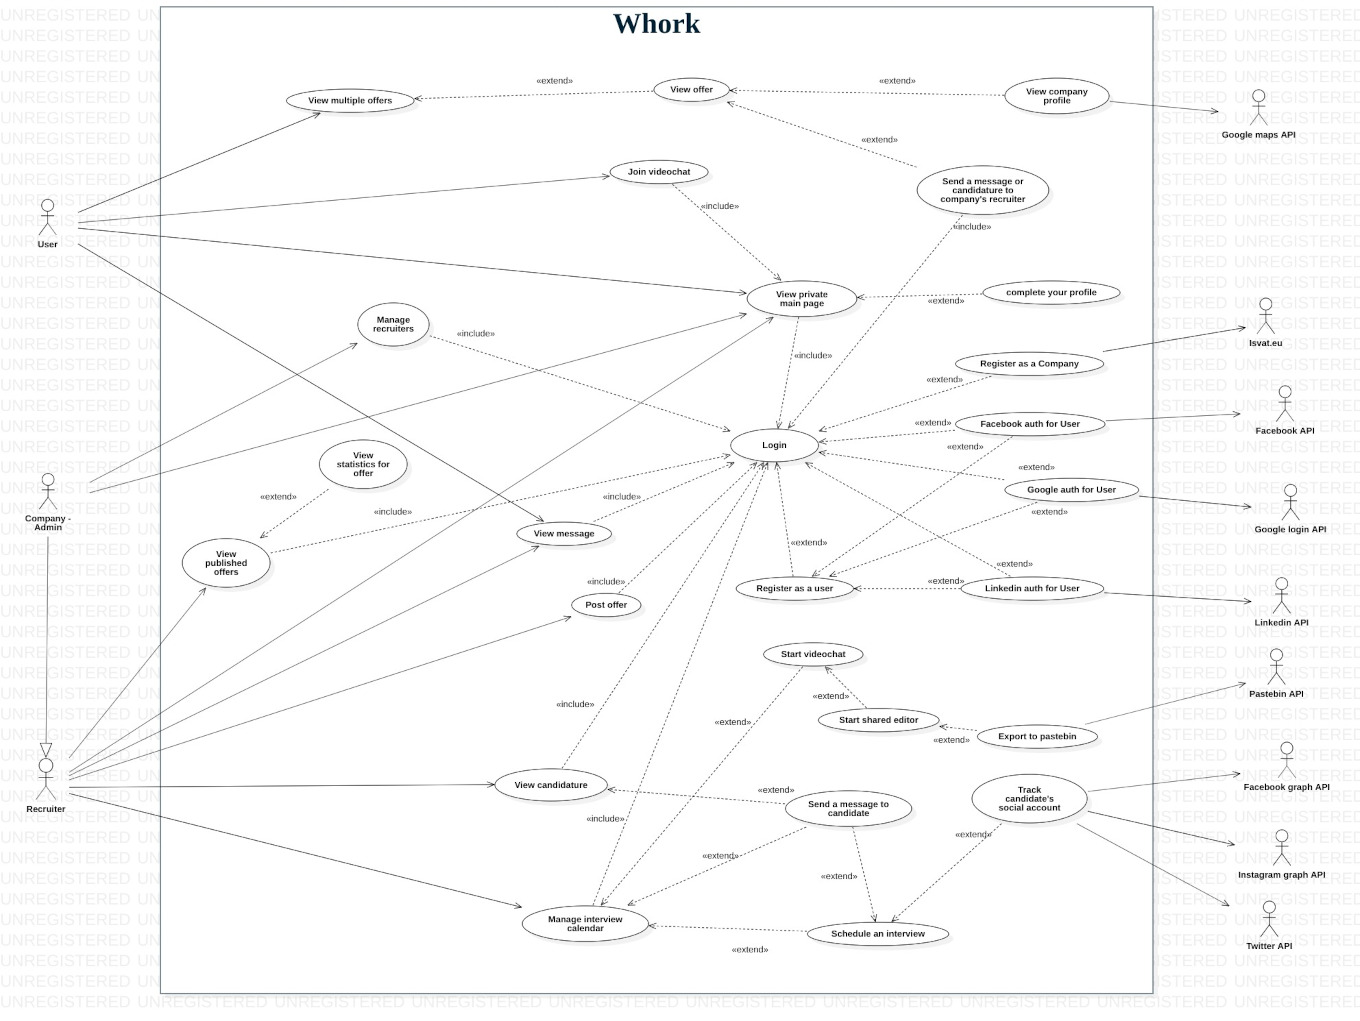
\includegraphics{diagrams/project/usecase/usecase_scaled.jpg}
\end{center}

\end{document}
